\documentclass{beamer}

\usepackage[orientation=landscape,size=a0,scale=1.4,debug]{beamerposter}
\mode<presentation>{\usetheme{mlr}}

\usepackage[sfdefault]{roboto}
\usepackage{roboto-mono}
\usepackage[T1]{fontenc}
\usepackage[utf8]{inputenc} % UTF-8
\usepackage[english]{babel} % Language
\usepackage{hyperref} % Hyperlinks
\usepackage{ragged2e} % Text position
\usepackage[export]{adjustbox} % Image position
\usepackage[most]{tcolorbox} % Code boxes
\usepackage{multido}

\hypersetup{
    hyperfootnotes=false,
    colorlinks=true,
	linktocpage=true,
	pdfauthor={mlr-org team},
    %linkcolor=[RGB]{3,99,142}, % mlr blue
    urlcolor=[RGB]{231,138,69}
}

\title{Machine learning with mlr3 :\,: CHEAT SHEET} % Package title in header, \, adds thin space between ::

\newlength{\columnheight} % Adjust depending on header height
\setlength{\columnheight}{84cm}

\newtcolorbox{codebox}{%
	sharp corners,
	leftrule=0pt,
	rightrule=0pt,
	toprule=0pt,
	bottomrule=0pt,
	fontupper=\robotomono\small,
	hbox}

\newtcolorbox{codeboxmultiline}[1][]{%
	sharp corners,
	leftrule=0pt,
	rightrule=0pt,
	toprule=0pt,
	bottomrule=0pt,
	fontupper=\robotomono\small,
	#1}

\newtcolorbox{codeboxexample}{%
	sharp corners,
	leftrule=0pt,
	rightrule=0pt,
	toprule=0pt,
	bottomrule=0pt,
	fontupper=\robotomono\small,
	width=27cm,
	adjusted title=Example,
	fonttitle = \bfseries\Large,
	top = 0.5em}

\newtcolorbox{codeboxinline}{%
	sharp corners,
	leftrule=0pt,
	rightrule=0pt,
	toprule=0pt,
	bottomrule=0pt,
	hbox,
	nobeforeafter,
	fontupper=\robotomono\small,
	tcbox raise base}

\newcommand{\codeinline}[1]{\begin{codeboxinline}#1\end{codeboxinline}}
\newcommand{\monospace}[1]{\multido{}{#1}{\space}}

\begin{document}
\begin{frame}[fragile]{}
	\begin{columns}
		\begin{column}{.245\textwidth}
			\begin{beamercolorbox}[center]{postercolumn}
				\begin{minipage}{.98\textwidth}
					\parbox[t][\columnheight]{\textwidth}{
						\begin{myblock}{Intro}
							The \textbf{mlr3} package builds on R6 classes and provides the essential building
							blocks of a machine learning workflow.
						\end{myblock}
						\begin{myblock}{mlr3 Dictionaries}
                            Key-value store for sets of mlr objects. These are provided by mlr3: 
							\vspace{0.5em}
							\begin{itemize}
								\item \codeinline{mlr\_tasks} - ML example tasks.
								\item \codeinline{mlr\_task\_generators} - Example generators.
                                \item \codeinline{mlr\_learners} - ML algorithms. 
								\item \codeinline{mlr\_measures} - Performance measures.
								\item \codeinline{mlr\_resamplings} - Resampling strategies.
							\end{itemize}
							\vspace{0.5em}
                            They can be extended and other dicts can be added by extension packages.
                            \codeinline{mlr\_learners} is populated by loading \textbf{mlr3learners} and other learner packages. Syntactic sugar functions retrieve objects from dicts, set hyperparameters and assign to fields in one go e.g. \codeinline{lrn(.key, ...)}.
							\\
							\begin{codebox}
								Dictionary\$\textbf{keys}(pattern = NULL)
							\end{codebox}
							Returns all keys which match \codeinline{pattern}. 
							If \codeinline{NULL}, all keys are returned. 
							\\
							\begin{codebox}
								Dictionary\$\textbf{get}(key, ...)
							\end{codebox}
							Retrieves object by \codeinline{key} and 
							passes arguments \codeinline{...} to the construction of the objects.
							\\
							\begin{codebox}
								Dictionary\$\textbf{mget}(keys, ...)
							\end{codebox}
							Retrieves objects by \codeinline{keys} and 
							passes named arguments \codeinline{...} to the construction of the objects. 
							\\
							\begin{codebox}
								as.data.table(Dictionary)
							\end{codebox}
							Lists objects with meta-data.
						\end{myblock}
					\vfill}
				\end{minipage}
			\end{beamercolorbox}
		\end{column}
		\begin{column}{.245\textwidth}
			\begin{beamercolorbox}[center]{postercolumn}
				\begin{minipage}{.98\textwidth}
					\parbox[t][\columnheight]{\textwidth}{
						\begin{myblock}{Task Class}
							Stores observation and columns (\codeinline{backend}) and additional
							meta-data about the dataset.
							\\
							\begin{codebox}
								task = \textbf{TaskClassif}\$new(backend, target)
							\end{codebox}
							For classification, \codeinline{target} needs to be a character vector representing class labels.
							\\
							\begin{codebox}
								task\$\textbf{positive} = "<positive\_class>"
							\end{codebox}
							Set positive class for binary classification.
							\\
							\begin{codebox}
								task = \textbf{TaskRegr}\$new(backend, target)
							\end{codebox}
							For regression, \codeinline{target} needs to be a numeric vector.
							\vspace{1em}
							\\
	                        Get example tasks with \codeinline{tsk(.key)}.
							\vspace{1em}
							\\
							Column roles affect the behavior of the task for different operations. Set with \codeinline{task\$\textbf{col\_roles}\$<role> = "<column\_name>"}:
							\\
							\begin{itemize}
								\item \codeinline{feature} - Regular features
								\item \codeinline{target} - Target variable
								\item \codeinline{name} - Labels for plots
								\item \codeinline{group} -  Groups for resampling
								\item \codeinline{stratum} - Stratification variables
								\item \codeinline{weight} - Observation weights
							\end{itemize}
							\vspace{1em}
							\begin{codebox}
								task\$\textbf{select}(cols)
							\end{codebox}
							Subsets the task based on feature names.
							\\
							\begin{codebox}
								task\$\textbf{filter}(rows)
							\end{codebox}
							Subsets the task based on row ids.
							\\
							\begin{codebox}
								task\$\textbf{cbind}(data)
							\end{codebox}
							Adds additional columns.
							\\
							\begin{codebox}
								task\$\textbf{rbind}(data)
							\end{codebox}
							Adds additional rows.
							\\
							\begin{codebox}
								task\$\textbf{rename}(from, to)
							\end{codebox}
							Rename columns.
						\end{myblock}
					\vfill}
				\end{minipage}
			\end{beamercolorbox}
		\end{column}
		\begin{column}{.245\textwidth}
			\begin{beamercolorbox}[center]{postercolumn}
				\begin{minipage}{.98\textwidth}
					\parbox[t][\columnheight]{\textwidth}{
						\begin{myblock}{Learner Class}
							Wraps learners from R with a unified interface.
							\\
							\begin{codebox}
								learner = \textbf{lrn}(.key, ...)
							\end{codebox}
							Get learner by \codeinline{.key} (from \codeinline{mlr\_learners}) 
							and construct the learner with specific hyperparameters and settings (...) in one go.
							\\
							\vspace{1em}
							\begin{codebox}
								learner\$\textbf{param\_set}
							\end{codebox}
							Returns description of hyperparameters.	
							\\
							\begin{codebox}
								learner\$param\_set\$\textbf{values} = list(id = value)
							\end{codebox}
							Change the current hyperparameter values by assigning a named \codeinline{list(id = value)} to the \codeinline{\$values} field.
							This overwrites all previously set parameters.	
							\\
							\begin{codebox}
								learner\$param\_set\$\textbf{values}\$<id> = <value>
							\end{codebox}
							Updates single hyperparameter.
							\vspace{1em}
							\\
							\begin{codebox}
								learner\$\textbf{predict\_type} = "<type>"
							\end{codebox}
							Changes what is technically output during prediction. For classification, 
	                        \codeinline{"response"} means class labels, \codeinline{"prob"} means posterior probabilities.
	                        For regression, \codeinline{"response"} means numeric response, 
	                        \codeinline{"se"} extracts the standard error.
							\vspace{1em}
							\begin{codeboxexample}
								{\scriptsize
									task = tsk("sonar")\\
									learner = lrn("classif.rpart")
									\vspace{1em}
									\\
									train\_set = sample(task\$nrow, 0.8 * task\$nrow)\\
									test\_set = setdiff(seq\_len(task\$nrow), train\_set)
									\vspace{1em}
									\\
									learner\$train(task, row\_ids = train\_set)
									\vspace{1em}
									\\
									prediction = learner\$predict(task, row\_ids = test\_set)\\
									prediction\$score()\\
									\#\# classif.ce\\
									\#\# \space 0.2619048}
							\end{codeboxexample}
						\end{myblock}
					\vfill}
				\end{minipage}
			\end{beamercolorbox}
		\end{column}
		\begin{column}{.245\textwidth}
			\begin{beamercolorbox}[center]{postercolumn}
				\begin{minipage}{.98\textwidth}
					\parbox[t][\columnheight]{\textwidth}{
						\begin{myblock}{Train \& Predict}
							\begin{codebox}
								learner\$\textbf{train}(task, row\_ids)
							\end{codebox}
	                        Train on (selected) observations. 
	                        The underlying R model is modified in place. 
							\\
							\begin{codebox}
								learner\$\textbf{model}
							\end{codebox}
							Retrieves the fitted R model.
							\\
							\vspace{1em} % Group Predict
							\begin{codebox}
								prediction = learner\$\textbf{predict}(task, row\_ids)
							\end{codebox}
	                        Predict (selected) observations.
	                        \\
	                        \begin{codeboxmultiline}[width=23cm]
								{\footnotesize prediction\\
								\#\# <PredictionClassif> for 42 observations:\\
								\#\# row\_id truth response\\
								\#\# \space\space\space\space\space 2
								\space\space\space\space R \space\space\space\space\space\space\space M\\
								\#\# \space\space\space\space\space 3
								\space\space\space\space R \space\space\space\space\space\space\space M\\
								\#\# \space\space\space\space\space 5
								\space\space\space\space R \space\space\space\space\space\space\space M\\
								\#\# - - -\\
								\#\# \space\space\space 198
								\space\space\space\space M \space\space\space\space\space\space\space M\\
								\#\# \space\space\space 200
								\space\space\space\space M \space\space\space\space\space\space\space M\\
								\#\# \space\space\space 207
								\space\space\space\space M \space\space\space\space\space\space\space M}
	                        \end{codeboxmultiline}
							\vspace{1em}
							\begin{codebox}
								prediction\$\textbf{data\$tab}
							\end{codebox}
							Returns predictions as \codeinline{data.table}.
	                    \end{myblock}
	                    \begin{myblock}{Measures \& Scoring}
							\begin{codebox}
								measure = \textbf{msr}(.key)
							\end{codebox}
							Get measure by \codeinline{.key} from \codeinline{mlr\_measures}.
							\\
							\begin{codebox}
								prediction\$\textbf{score}(measure)
							\end{codebox}
							Access performance with \codeinline{measure}.
						\end{myblock}
					\vfill}
				\end{minipage}
			\end{beamercolorbox}
		\end{column}
	\end{columns}
\end{frame}
\begin{withoutheader}
\begin{frame}[fragile]{}
	\begin{columns}
		\begin{column}{.245\textwidth}
			\begin{beamercolorbox}[center]{postercolumn}
				\begin{minipage}{.98\textwidth}
					\parbox[t][\columnheight]{\textwidth}{
						\begin{myblock}{Resampling Class}
							Define later partitioning of task into series of train and test sets. \\ 
							Create with \codeinline{resampling = \textbf{rsmp}(.key, ...)}:
							\\
							\begin{itemize}
                                \item \codeinline{holdout}
                                (\codeinline{ratio})\\
                                Holdout-validation.
								\item \codeinline{cv}
								(\codeinline{folds})\\
								k-fold cross-validation.
								\item \codeinline{repeated\_cv}
								(\codeinline{folds}, \codeinline{repeats})\\
								Repeated k-fold cross-validation.
								\item \codeinline{subsampling}
								(\codeinline{repeats}, \codeinline{ratio})\\
								Repeated holdouts.
								\item \codeinline{bootstrap}
								(\codeinline{repeats}, \codeinline{ratio})\\
								Out-of-bag bootstrap.
								\item Custom splits \\
							\begin{codeboxmultiline}[width=26cm]
							resampling = rsmp("\textbf{custom}")\\
							resampling\$instantiate(task,\\
							\hspace*{1ex} train = list(c(1:10, 51:60, 101:110)),\\
							\hspace*{1ex} test = list(c(11:20, 61:70, 111:120)))
							\end{codeboxmultiline}
							\end{itemize}
							\vspace{1em}
							\begin{codebox}
								resampling\$\textbf{param\_set}
							\end{codebox}
							Returns a description of parameter settings.
							\\
							\begin{codebox}
								{\footnotesize resampling\$param\_set\$\textbf{values} = list(folds = 10)}
							\end{codebox}
							Sets folds to 10.
							\\
							\begin{codebox}
								task\$col\_roles\$\textbf{stratum} = "<column\_names>"
							\end{codebox}
							Sets stratification variables.
							\\
							\begin{codebox}
								task\$col\_roles\$\textbf{group} = "<column\_name>"
							\end{codebox}
							Sets group variable.
							\\
							\begin{codebox}
								resampling\$\textbf{instantiate}(task)
							\end{codebox}
                            Perform splitting and define index sets.
                            \vspace{1em}
							\\
							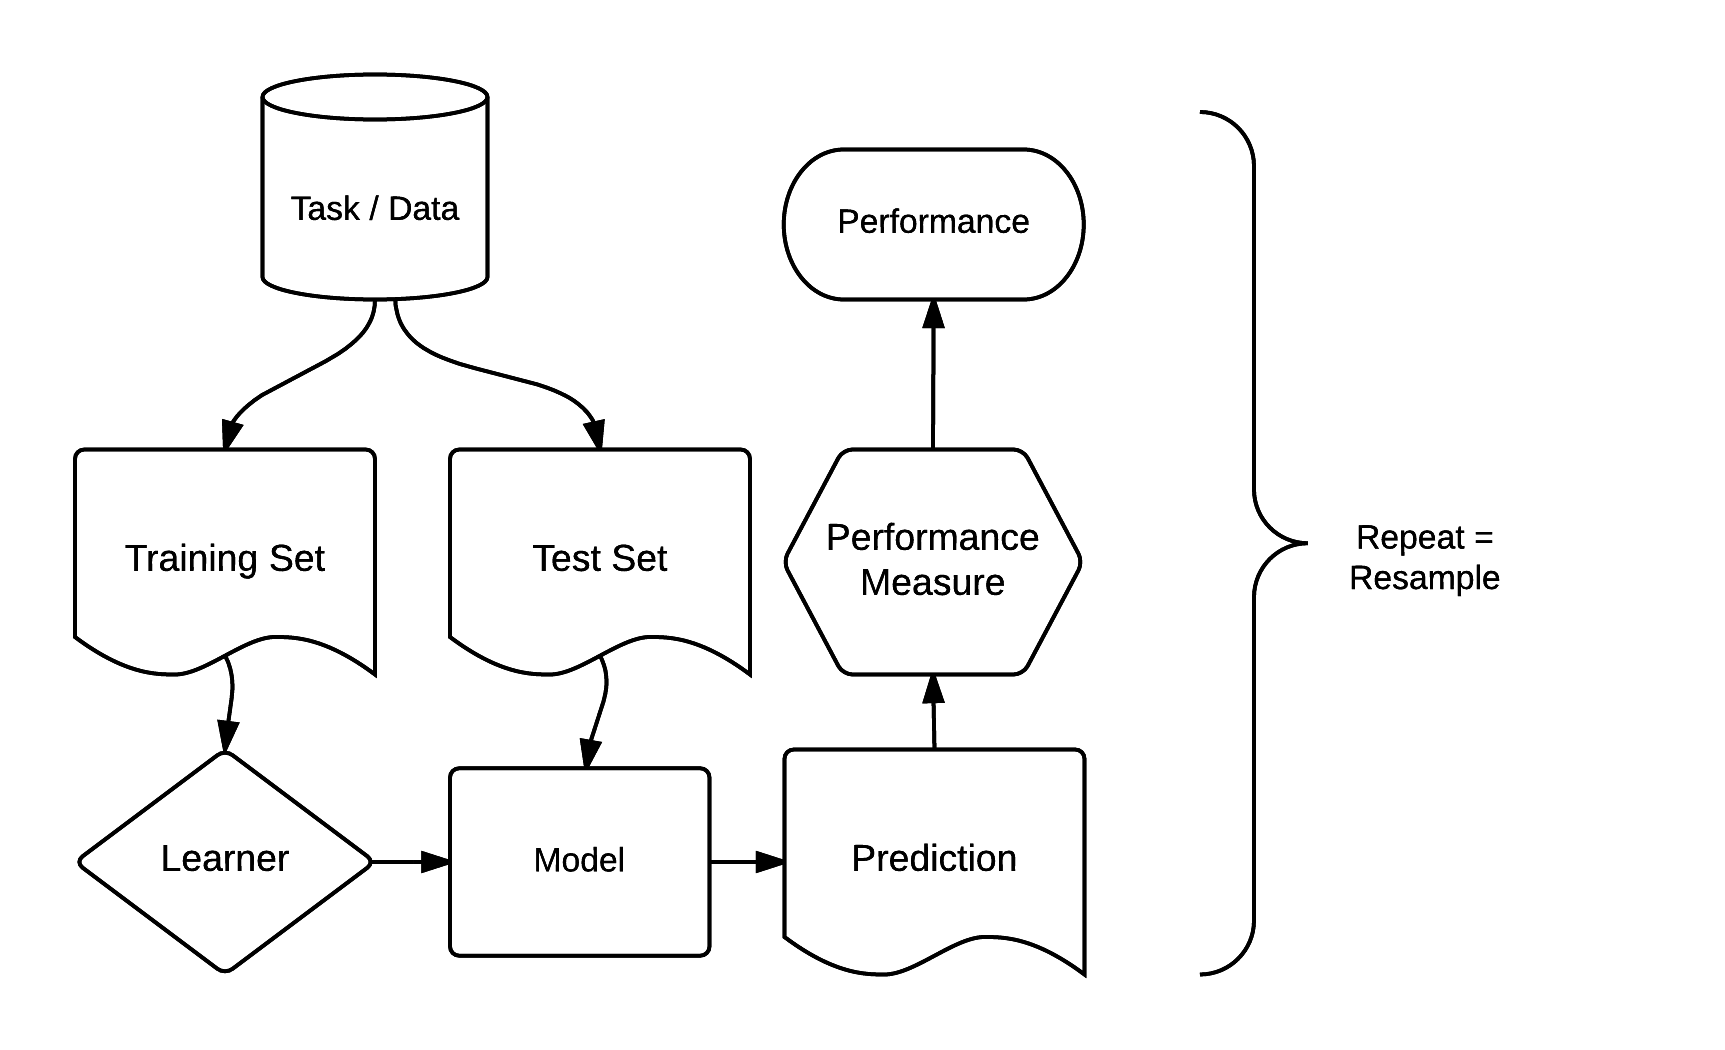
\includegraphics[width=\textwidth]{img/ml_abstraction.png}
							\\
						\end{myblock}
					\vfill}
				\end{minipage}
			\end{beamercolorbox}
		\end{column}
		\begin{column}{.245\textwidth}
			\begin{beamercolorbox}[center]{postercolumn}
				\begin{minipage}{.98\textwidth}
					\parbox[t][\columnheight]{\textwidth}{
						\begin{myblock}{Resample}
                            Train-Predict-Score learner for each train/test set.
							\\
							\begin{codebox}
								rr = \textbf{resample}(task, learner, resampling)
							\end{codebox}
							Returns a \codeinline{ResampleResult} container object.
							\\
							\begin{codebox}
								rr\$\textbf{score}(measures)
							\end{codebox}
							Returns datatable of scores on test sets.
							\\
							\begin{codebox}
								rr\$\textbf{aggregate}(measures)
							\end{codebox}
						    Get aggregated performance scores as vector.
							\\
							\begin{codebox}
								rr\$\textbf{filter}(iters)
							\end{codebox}
							Reduces to iterations.
							\\
							\begin{codeboxexample}
								\scriptsize{
									task = tsk("pima")\\
									learner = lrn("classif.rpart", predict\_type = "prob")\\
									measure = msr("classif.ce")
									\vspace{1em}
									\\
									resampling = rsmp("cv", folds = 3L)\\
									resampling\$instantiate(task)
									\vspace{1em}
									\\
									rr = resample(task, learner, resampling)
									\vspace{1em}
									\\
									rr\$data\\
									\#\# ...\monospace{3}resampling iteration prediction\\
									\#\# ... <ResamplingCV>\monospace{9}1\monospace{5}<list>\\
									\#\# ... <ResamplingCV>\monospace{9}2\monospace{5}<list>\\
									\#\# ... <ResamplingCV>\monospace{9}3\monospace{5}<list>
									\vspace{1em}
									\\
									rr\$aggregate(measure)\\
									\#\# classif.ce\\
									\#\# \monospace{4}0.2643
									\vspace{1em}
									\\
									learners = lrns(c("classif.rpart", "classif.ranger"))\\
									tasks = tsks(c("sonar", "spam"))\\
									resampling = rsmp("cv", folds = 3L)
									\vspace{1em}
									\\
									design = benchmark\_grid(tasks, learners,resampling)
									\vspace{1em}
									\\
									bmr = benchmark(design)\\
									bmr\\
									\#\# <BenchmarkResult> of 12 rows with 4 resampling runs\\
									\#\# nr task\_id\monospace{5}learner\_id resampling\_id iters ...\\
									\#\#\monospace{2}1\monospace{3}sonar\monospace{2}classif.rpart
									\monospace{12}cv\monospace{4}3 ...\\
									\#\#\monospace{2}2\monospace{3}sonar classif.ranger
									\monospace{12}cv\monospace{4}3 ...\\
									\#\#\monospace{2}3\monospace{4}spam\monospace{2}classif.rpart
									\monospace{12}cv\monospace{4}3 ...\\
									\#\#\monospace{2}4\monospace{4}spam classif.ranger
									\monospace{12}cv\monospace{4}3 ...
									\vspace{1em}
									\\
									bmr\$aggregate()\\
									\#\# nr \monospace{2}resample\_result ... classif.ce\\
									\#\#\monospace{2}1\monospace{2}<ResampleResult> ... 0.26928916\\
									\#\#\monospace{2}2\monospace{2}<ResampleResult> ... 0.17798482\\
									\#\#\monospace{2}3\monospace{2}<ResampleResult> ... 0.10106500\\
									\#\#\monospace{2}4\monospace{2}<ResampleResult> ... 0.10106500}
							\end{codeboxexample}
							Results are presented in datatables.
							\codeinline{BenchmarkResult} contains a \codeinline{ResampleResult} for each task-learner-resampling combination
							which in turn contain a \codeinline{Prediction} for each resampling iteration.
						\end{myblock}
					\vfill}
				\end{minipage}
			\end{beamercolorbox}
		\end{column}
		\begin{column}{.245\textwidth}
			\begin{beamercolorbox}[center]{postercolumn}
				\begin{minipage}{.98\textwidth}
					\parbox[t][\columnheight]{\textwidth}{
						\begin{myblock}{Benchmark}
                            Compare learner(s) on task(s) with resampling(s).
							\\
							\begin{codeboxmultiline}[width=19.4cm]
								design = \textbf{benchmark\_grid}(\\
								\hspace*{1ex}tasks, learners, resamplings)
							\end{codeboxmultiline}
							Creates a cross-join datatable with list-cols, you can also manually define this for full control.
							\\
							\begin{codebox}
								bmr = \textbf{benchmark}(design)
							\end{codebox}
							Returns a \codeinline{\robotomono{BenckmarkResult}}
							container.
							\\
							\begin{codebox}
								bmr\$\textbf{aggregate}(measures)
							\end{codebox}
							Datatable of ResampleResults with scores.
							\\
							\begin{codebox}
								bmr\$\textbf{score}(measures)
							\end{codebox}
							Datatable of resampling iterations with scores. 
							\\
							\begin{codeboxmultiline}[width=21.5cm]
								bmr\$\textbf{filter}(task\_ids, learner\_ids,\\ 
								\hspace*{1ex}resampling\_ids)
							\end{codeboxmultiline}
							Filter by task, learner and resampling. 
							\\
							\begin{codebox}
								bmr\$\textbf{combine}(bmr)
							\end{codebox}
							Fuse a second \codeinline{BenchmarkResult}. 
						\end{myblock}
						\begin{myblock}{Parallelization}
							\codeinline{future} is used as backend for parallelization.
							\\
							\begin{codebox}
								future::\textbf{plan}(strategy)
							\end{codebox}
							Selects the parallelization strategy. 
							All operations building on top of the \codeinline{resample()} function 
							such as resampling, benchmarking, tuning and feature selection are executed in parallel.
						\end{myblock}
						\begin{myblock}{mlr3viz}
							Provides visualization for mlr3 objects.
							Create with \codeinline{mlr3viz::autoplot(object, type)}
							\\
							\begin{itemize}
								\item \codeinline{BenchmarkResult} (\codeinline{boxplot}, \codeinline{roc}, \codeinline{prc})
								\item \codeinline{Filter} (\codeinline{barplot})
								\item \codeinline{PredictionClassif} (\codeinline{stacked}, \codeinline{roc}, \codeinline{prc})
								\item \codeinline{PredictionRegr} (\codeinline{xy}, \codeinline{histogram})
								\item \codeinline{ResampleResult} (\codeinline{boxplot}, \codeinline{histogram}, \codeinline{roc}, \codeinline{prc})
								\item \codeinline{TaskClassif} (\codeinline{target}, \codeinline{duo}, \codeinline{pairs})
								\item \codeinline{TaskRegr} (\codeinline{target}, \codeinline{pairs})
								\item \codeinline{TaskSurv} (\codeinline{target}, \codeinline{duo}, \codeinline{pairs})
							\end{itemize}
						\end{myblock}
					\vfill}
				\end{minipage}
			\end{beamercolorbox}
		\end{column}
		\begin{column}{.245\textwidth}
			\begin{beamercolorbox}[center]{postercolumn}
				\begin{minipage}{.98\textwidth}
					\parbox[t][\columnheight]{\textwidth}{
						\begin{myblock}{Logging}
							\codeinline{lgr} is used for logging and progress output.
							\\
							\begin{codeboxmultiline}[width=23.1cm]
								\textbf{getOption}("lgr.log\_levels")\\
								\#\# fatal error  warn  info debug trace\\ 
								\#\# 100\monospace{3}200\monospace{3}300\monospace{2}400\monospace{2}500\monospace{3}600
							\end{codeboxmultiline}
							Gets threshold levels. The default is 400. 
							\\
							\begin{codeboxmultiline}[width=25cm]
								\footnotesize{
								lgr::get\_logger("mlr3")\$\textbf{set\_threshold}("<level>")}
							\end{codeboxmultiline}
							Change log-level, you can also do this for other mlr3 packages analogously.
						\end{myblock}
						\begin{myblock}{Error Handling and Encapsulation}
							The \codeinline{evaluate} package is used to encapsulate execution of \codeinline{\$train} and \codeinline{\$predict} to prevent the program flow from stopping in case of errors, warnings and crashes.
							\\
							\begin{codeboxmultiline}[width=16cm]
								learner\$\textbf{encapsulate} = c(\\
								\hspace*{1ex} train = "evaluate", \\
								\hspace*{1ex} predict = "evaluate")
							\end{codeboxmultiline}
							\vspace{1em}
							\begin{codebox}
								learner\$\textbf{errors}
							\end{codebox}
							Access the recorded log of errors.
							\\
							\begin{codebox}
								learner\$\textbf{fallback} = lrn(.key)
							\end{codebox}
							If learner fails, fallback is used to generate predictions. 
                            Use robust fallback, e.g. "featureless"! Can ease pain in complex benchmarks when learners fail in edge-cases.
						\end{myblock}
						\begin{myblock}{Resources}
							\begin{itemize}
								\item \href{https://mlr3book.mlr-org.com/index.html}{mlr3book}\\ (https://mlr3book.mlr-org.com)
								\item \href{https://github.com/mlr-org}{mlr-org on GitHub}\\ (https://github.com/mlr-org)
								\item \href{https://github.com/mlr-org/mlr3learners}{mlr3learners package}\\ (https://github.com/mlr-org/mlr3learners)
								\item \href{https://github.com/mlr3learners}{mlr3learners organization}\\ (https://github.com/mlr3learners)
							\end{itemize}
						\end{myblock}
					\vfill}
				\end{minipage}
			\end{beamercolorbox}
		\end{column}
	\end{columns}
\end{frame}
\end{withoutheader}
\end{document}
